\documentclass{article}
\usepackage[utf8]{inputenc}
\usepackage[a4paper, margin=1in]{geometry}
\usepackage[font={small,it}]{caption}
\usepackage{graphicx}
\usepackage{xcolor}
\usepackage{pdfpages}
\usepackage{natbib}
\usepackage{graphicx}
\usepackage{float}
\usepackage{url}
\usepackage{nameref}
\usepackage{pdflscape}
\usepackage{listings}
\usepackage{xparse}
\graphicspath{{../Figures/}}
\bibliographystyle{agsm}
\NewDocumentCommand{\codeword}{v}{%
\texttt{{#1}}%
}
\lstset{language=C,keywordstyle={\bfseries}}

\title{\textbf{Examining the Effects of Advanced Programming Constructs}}
\author{
Luca Davies \\ M.Sci. (Hons.) Computer Science (with Industrial Experience)}
\date{4th June 2021}

\begin{document}
\maketitle

\newpage
\section*{Declaration}
    I certify that the material contained in this dissertation is my own work and does not contain unreferenced or unacknowledged material. I also warrant that the above statement applies to the implementation of the project and all associated documentation. Regarding the electronically submitted work, I consent to this being stored electronically and copied for assessment purposes, including the School’s use of plagiarism detection systems in order to check the integrity of assessed work. \\
    I agree to my dissertation being placed in the public domain, with my name explicitly included as the author of the work. \\
    
    \noindent
    Name: Luca Davies\\
    Date: 01/06/2021
\newpage
\section*{Abstract}
    As time has gone on, languages have become more developed themselves more advanced syntax constructs have been added alongside many "quality of life" type structures to make the writing code not only more efficient but also easier for developers. This report examines a number of these advanced constructs, drawing together both data from surveys taken by professional developers and data from analysis of a small number of large, active, open source code bases. Using a short but broad survey, data was collected on developers usage of these constructs and they provided information on how they felt these constructs affected their code and how often they used them, and how they thought they existed within the context of the wider industry. Analysis of code was carried using a combination of both simple regular expressions and via the user of lightweight tool to aid in the bulk processing of a large volume of source code file. It was found that ... don't know yet. FINISH ABSTRACT.
    \newline
    \newline
    [Is there any working docs?]
\newpage
\tableofcontents
\newpage

% https://www.joelonsoftware.com/2005/05/11/making-wrong-code-look-wrong/

\section{Introduction}
    \subsection{Overview}
    \label{sec:overview}
        Programming as we know it today - in terms of high-level languages - has been around for over half a century. From FORTRAN in 1957, to Java in 1995, to Swift in 2014, the languages we use to power our ever-growing number of devices have been getting more and more powerful themselves. The tools we have now allow us to do things that would have been thought impossible 50 years ago. Programs that may have used 1000 lines to perform maintenance on a device in '60s, can now be written to maintain devices running thousands of times faster \emph{and} take care of many many more tasks... all in the same number of lines. More and more we're also depending on our programming, a degree of code will be involved in nearly any electronic device you can use today, and not just those devices in domestic settings, but also those piloting our aircraft and cars and keeping our electricity network functioning.

        It's easy to see why then, that the ease of \emph{anything and everything} in programming is extremely valuable. There is thus an incentive to keep our programming languages simple. If a set a rules is very simple and easy to understand, it should be equally easy to abide by them and prevent mistakes - however, if that were the case, why would ever have left machine code or assembly language behind? They are simple, but that is also their downfall. Putting together a large simple program in this way become for too complex for the average programmer to keep in their head while programming, and there's no question that it's tougher to spot mistakes when your code is only half human-readable. So we can amend our axiom of simplicity to not be in the nature of the language itself, but in our interactions with the language: the easier we can make it to write our code, read our code, check our code, the lesser the chance of a mistake making it on to a production device and causing damage or harm. 

        This is exactly what we have seen happen over time. As languages do become more complex, the hope is that they become easier and easier for a programmer to use. Available syntax was once only of the form \codeword{command operand}, but now there's a myriad of complex but highly useful syntax and control flow structures to make the life of a developer much easier than it may have otherwise been. Though flow-control remains a key part of imperative languages, some declarative languages need not even define \emph{how} something is done, simply \emph{what} must be done. In imperative languages there are still abstractions of another type: those constructs that take existing syntax and functionality and compound it into a singular construct that programmers may use as a form of short-hand. 
        
        It is these constructs that this paper examines, using C\#, JavaScript, and Java as a representative sample of popular imperative programming languages. Namely we will be focussing on the following constructs and their usage in these languages:
        
        \begin{itemize}
            \item Ternary/in-line If Statements ( \codeword{a ? b : c} )
            \item Null-coalesce ( \codeword{a ?? b} ) and Null-conditional Operators ( \codeword{a?.b} / \codeword{a?[x]b})
            \item Lambda Expressions and Anonymous Functions ( \codeword{(a) => { b; }} )
            \item Additional constructs:
            \begin{itemize}
                \item Foreach Loops ( \codeword{foreach (a in b)} / \codeword{for ( a : b )})
                \item Unary Increment Operators (\codeword{a++}, \codeword{b--})
                \item Compound Assignment Operators (\codeword{a += 2},  \codeword{b -= 2}, \codeword{c *= 2}, \codeword{d /= 2}, etc...)
            \end{itemize}
        \end{itemize}
        
        \emph{Detailed descriptions of these constructs are given in section \ref{sec:dunno}}\\

        They may be used for multiple reasons, such as to make code simpler, or clearer. Other times, it may be style defined either by a programmer themselves, or the house rules of their organisation. No tool however it unable to be misused - overuse of these types of constructs or use of them in inappropriate places can in fact make code more complicated and harder to read than it would have been using more basic syntax. In this paper, we will study the above constructs and how they are used, with a view to making recommendations about they are best used, and where they are best avoided.
    \subsection{Motivation}
        The primary drive for this study came from my experience during my industrial placement (SCC.419). The codebase I was working on was extensive and developed by numerous developers over the course of the last two decades or so. There were times that code was either made easier or harder not by its flow, but by the way it was written. The first instance that came to my attention was a ternary if-statement used that was so long that it needed to be split across four lines, had a second and third ternary in the true \emph{and} false branch of the enclosing ternary, with lengthy expressions being evaluated from there. In this instance, it would have been significantly clearer to use a regular if-statement. Despite this the existence of ternary if-statements is still useful, but it brings to question where these constructs and other similar constructs should best be used.

        There also seems to have been relatively little research into languages features such as that which will be examined here, either in terms of subjective readability or objective performance. It is hoped that by formally examining some of these constructs in a small selection of languages that the contribution provided will, if not self-contained, provide a launch pad for more thorough examination.
    \subsection{Aims \& Objectives}
        The aims of this report are as follows:
        \begin{itemize}
            \item To identify and understand the usage of a selection of advanced programming constructs (as defined in sections \ref{sec:overview} and \ref{subsec:constructs})
            \item aha
            \item 
        \end{itemize}
    \subsection{Report Structure}
        The remainder of this report will discuss ...
\newpage
\section{Background}
\label{sec:background)}
Some text
\begin{landscape}
    \begin{figure}[htbp]
        \centering
        \vspace{2in}
        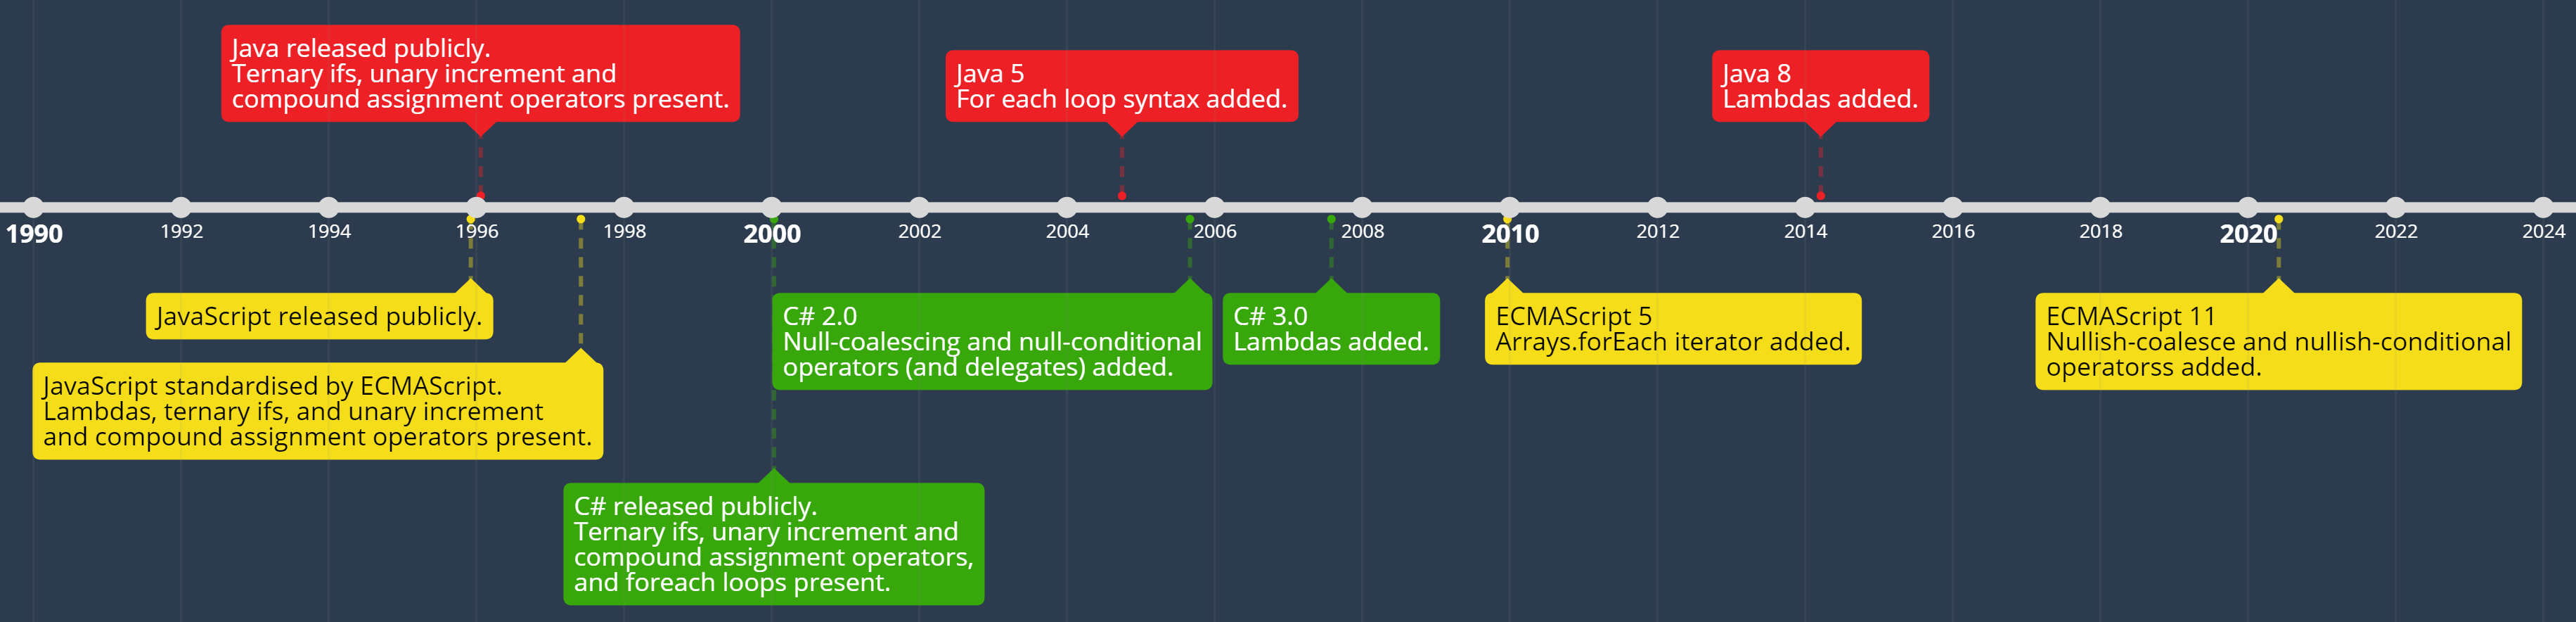
\includegraphics[width=1.5\textheight]{timeline}
        \caption{Timeline of the addition of advanced constructs to three modern languages.}
        \label{fig:timeline}
    \end{figure}
\end{landscape}
\section{Study Design}
    \subsection{Constructs}
    \label{subsec:constructs}
    Need this in detail somewhere.
    \begin{itemize}
        \item Ternary/in-line If Statements
            \begin{itemize}
                \item Reduces the common \codeword{if} \dots \codeword{else} \dots pattern into a single line of the form \codeword{a ? b : c}, where \codeword{a} is a conditional expression, \codeword{b} is the body of the \codeword{if} and \codeword{c} is the body of the \codeword{else}.
            \end{itemize}
        \item Lambdas and Anonymous Functions
            \begin{itemize}
                \item A lambda expression is any expression involving a function used as an argument, just as in Lambda Calculus. Though this is not required, lambdas most often take the form of anonymous (unnamed) functions defined in-line. \citep{javaLambdas}
            \end{itemize}
        \item Null-coalescing Operator
            \begin{itemize}
                \item Used to provide a default value in place of a null value. Replaces a null-check (using an if statement) with a single assignment of the form \newline\codeword{a = possiblyNullValue  ?? valueIfNull} where \codeword{a} is of a nullable type. \citep{gunnerson2012programmer}
            \end{itemize}
        \item Null-conditional Operator
         \item Foreach Loops
        \item Unary Increment Operator
        \item Compound Assignment Operators
    \end{itemize}

    \subsection{Survey}
        Using Qualtrics blah blah blah
        \subsubsection{Questions}
            The survey was designed to address the following questions:
            \begin{itemize}
                \item Are the participants \emph{aware} of the constructs?
                \item Do the participants \emph{use} the constructs?
                \item Are participants \emph{encouraged to use} the constructs?
                \item Do the participants think these constructs are better for:
                    \subitem brevity?
                    \subitem clarity?
                    \subitem efficiency/performance?
                \item Do the participants think that the constructs are better used in some languages than in others?
                \item Do participants rewrite code \emph{to use} or \emph{to not use} the constructs?
            \end{itemize}      
            
            Hypothesis/expected results
        \subsubsection{Participants}
            Who?
            Where from?
            How many?
        \subsubsection{Content}
            How are questions above addressed?
    \subsection{Static Code Analysis}
            Using multiple tools, which?
        \subsubsection{Sample Code Files}
            One per language, features examples of the basic and advanced form of all constructs
        \subsubsection{Open Source Repositories}
            Selection process?
            Big enough to assume reasonable presence of constructs
    \subsection{Git Commit Analysis}
        Keywords used
    
\section{Results}
    \subsection{Survey}
            []
    \subsection{Static Code Analysis}
        []
        \subsubsection{Sample Code Files}
            Bugger all picked up, tools do not care
            \begin{itemize}
                \item Picked up basic for in place of JS for-to (not for/each)
            \end{itemize}
        \subsubsection{Real-World Code Bases}
            []
\section{Conclusion}
\label{sec:conclusion}
    []
    \subsection{Review of Aims}
        The following list repeats the aims presented at the start of this report, with each aim followed by an overview of relevant results obtained.
        \begin{itemize}
            \item \textcolor{gray}{\textit{[]}}
                []
            \item \textcolor{gray}{\textit{[]}}
                []
            \item \textcolor{gray}{\textit{[]}}
                []
            \item \textcolor{gray}{\textit{[]}}
                []
            \item \textcolor{gray}{\textit{}}
                []
        \end{itemize}
    \subsection{Reflections}
        []
    \subsection{Negative Impacting Circumstances}
        The on-going coronavirus pandemic is still very much a factor in the lives us all. :(
    \subsection{Future Research}
        []
    \subsection{Closing Statement}
        []
\bibliography{ref}
\newpage
\section*{Appendix}
    \subsection*{Appendix 1: []}
        []
    \subsection*{Appendix 2: []}
        []
\end{document}
